\documentclass[10pt]{article}
\usepackage[paperwidth=11.8cm,paperheight=4.5cm,margin=0pt]{geometry}
\usepackage{amsmath,amssymb}
\usepackage{mathptmx}
\renewcommand{\hbar}{\mathchar'26\mkern-9mu h}
\usepackage{tikz}
\pagestyle{empty}
\begin{document}
\special{papersize=11.8cm,4.5cm}
\noindent
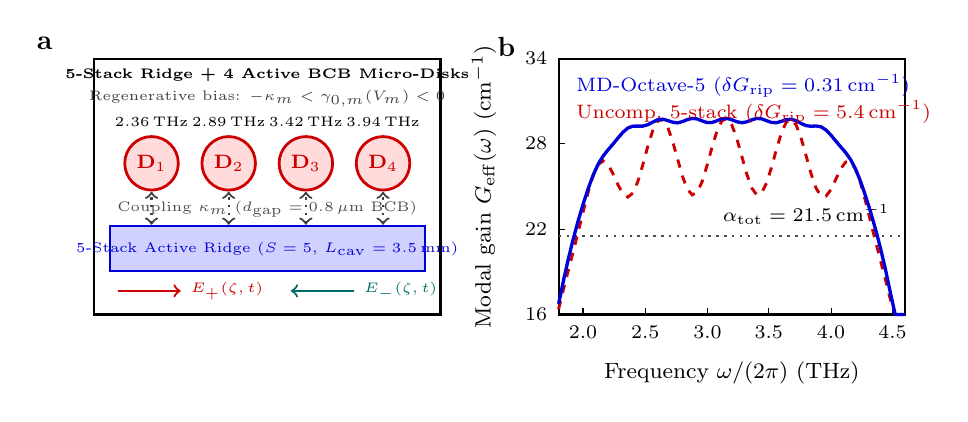
\begin{tikzpicture}[x=1cm,y=1cm,font=\footnotesize]
  % Panel a: Schematic of 5-stack ridge waveguide coupled to M=4 BCB micro-disks
  \node[anchor=north west,font=\bfseries\normalsize] at (0.10,4.35) {a};
  \draw[thick] (0.95,0.70) rectangle (5.35,3.95);
  \node[font=\tiny\bfseries] at (3.15,3.74) {5-Stack Ridge + 4 Active BCB Micro-Disks};

  % Main 5-stack ridge waveguide
  \fill[blue!18] (1.15,1.25) rectangle (5.15,1.82);
  \draw[blue!85!black,thick] (1.15,1.25) rectangle (5.15,1.82);
  \node[font=\tiny,blue!85!black] at (3.15,1.53) {5-Stack Active Ridge ($S=5$, $L_{\mathrm{cav}}=3.5\,\mathrm{mm}$)};
  \draw[->,red!80!black,thick] (1.25,1.00) -- (2.05,1.00) node[right,font=\tiny] {$E_+(\zeta,t)$};
  \draw[<-,teal!85!black,thick] (3.45,1.00) -- (4.25,1.00) node[right,font=\tiny] {$E_-(\zeta,t)$};

  % 4 evanescently coupled active micro-disks
  \foreach \xc/\lbl/\freq in {1.68/D$_1$/2.36, 2.66/D$_2$/2.89, 3.64/D$_3$/3.42, 4.62/D$_4$/3.94} {
    \fill[red!14] (\xc,2.62) circle (0.34cm);
    \draw[red!80!black,line width=1.0pt] (\xc,2.62) circle (0.34cm);
    \node[font=\scriptsize\bfseries,red!80!black] at (\xc,2.62) {\lbl};
    \node[above,font=\tiny] at (\xc,2.97) {$\freq\,\mathrm{THz}$};
    \draw[<->,dotted,black!75,thick] (\xc,1.84) -- (\xc,2.26);
  }
  \node[font=\tiny,black!75] at (3.15,3.44) {Regenerative bias: $-\kappa_m < \gamma_{0,m}(V_m) < 0$};
  \node[font=\tiny,black!70] at (3.15,2.04) {Coupling $\kappa_m$ ($d_{\mathrm{gap}}=0.8\,\mu\mathrm{m}$ BCB)};

  % Panel b: Bare 5-stack ripple vs Micro-disk flattened gain spectrum
  \node[anchor=north west,font=\bfseries\normalsize] at (5.95,4.35) {b};
  \draw[thick] (6.85,0.70) rectangle (11.25,3.95);
  \foreach \v/\y in {16/0.70, 22/1.78, 28/2.87, 34/3.95} {
    \draw (6.85,\y) -- (6.93,\y);
    \node[left,font=\scriptsize] at (6.83,\y) {\v};
  }
  \foreach \fval/\xpos in {2.0/7.16, 2.5/7.95, 3.0/8.74, 3.5/9.52, 4.0/10.31, 4.5/11.09} {
    \draw (\xpos,0.70) -- (\xpos,0.78);
    \node[below,font=\scriptsize] at (\xpos,0.68) {\fval};
  }
  \node[below,font=\footnotesize] at (9.05,0.22) {Frequency $\omega/(2\pi)$ (THz)};
  \node[rotate=90,above,font=\footnotesize] at (6.18,2.32) {Modal gain $G_{\mathrm{eff}}(\omega)$ ($\mathrm{cm}^{-1}$)};

  % Cavity threshold loss line
  \draw[dotted,black!70,line width=0.85pt] (6.85,1.70) -- (11.25,1.70);
  \node[anchor=south east,font=\scriptsize] at (11.18,1.72) {$\alpha_{\mathrm{tot}}=21.5\,\mathrm{cm}^{-1}$};

  \draw[red!80!black,dashed,line width=1.05pt] (6.850,0.768) -- (6.913,1.028) -- (6.976,1.272) -- (7.039,1.512) -- (7.101,1.760) -- (7.164,2.015) -- (7.227,2.261) -- (7.290,2.468) -- (7.353,2.605) -- (7.416,2.651) -- (7.479,2.603) -- (7.541,2.487) -- (7.604,2.347) -- (7.667,2.234) -- (7.730,2.191) -- (7.793,2.243) -- (7.856,2.389) -- (7.919,2.600) -- (7.981,2.832) -- (8.044,3.032) -- (8.107,3.156) -- (8.170,3.175) -- (8.233,3.085) -- (8.296,2.907) -- (8.359,2.681) -- (8.421,2.460) -- (8.484,2.293) -- (8.547,2.219) -- (8.610,2.253) -- (8.673,2.389) -- (8.736,2.596) -- (8.799,2.827) -- (8.861,3.030) -- (8.924,3.161) -- (8.987,3.188) -- (9.050,3.107) -- (9.113,2.935) -- (9.176,2.711) -- (9.239,2.486) -- (9.301,2.310) -- (9.364,2.222) -- (9.427,2.243) -- (9.490,2.367) -- (9.553,2.567) -- (9.616,2.797) -- (9.679,3.005) -- (9.741,3.143) -- (9.804,3.179) -- (9.867,3.106) -- (9.930,2.939) -- (9.993,2.717) -- (10.056,2.489) -- (10.119,2.305) -- (10.181,2.205) -- (10.244,2.202) -- (10.307,2.284) -- (10.370,2.417) -- (10.433,2.551) -- (10.496,2.637) -- (10.559,2.640) -- (10.621,2.547) -- (10.684,2.371) -- (10.747,2.141) -- (10.810,1.887) -- (10.873,1.635) -- (10.936,1.391) -- (10.999,1.151) -- (11.061,0.901) -- (11.124,0.700) -- (11.187,0.700) -- (11.250,0.700);
  \draw[blue!85!black,line width=1.2pt] (6.850,0.835) -- (6.913,1.137) -- (6.976,1.418) -- (7.039,1.672) -- (7.101,1.901) -- (7.164,2.111) -- (7.227,2.304) -- (7.290,2.474) -- (7.353,2.612) -- (7.416,2.714) -- (7.479,2.793) -- (7.541,2.865) -- (7.604,2.942) -- (7.667,3.015) -- (7.730,3.069) -- (7.793,3.092) -- (7.856,3.093) -- (7.919,3.093) -- (7.981,3.110) -- (8.044,3.143) -- (8.107,3.173) -- (8.170,3.181) -- (8.233,3.165) -- (8.296,3.143) -- (8.359,3.134) -- (8.421,3.149) -- (8.484,3.175) -- (8.547,3.191) -- (8.610,3.184) -- (8.673,3.159) -- (8.736,3.138) -- (8.799,3.139) -- (8.861,3.161) -- (8.924,3.185) -- (8.987,3.191) -- (9.050,3.174) -- (9.113,3.148) -- (9.176,3.136) -- (9.239,3.147) -- (9.301,3.172) -- (9.364,3.190) -- (9.427,3.186) -- (9.490,3.162) -- (9.553,3.139) -- (9.616,3.136) -- (9.679,3.153) -- (9.741,3.175) -- (9.804,3.180) -- (9.867,3.160) -- (9.930,3.126) -- (9.993,3.099) -- (10.056,3.091) -- (10.119,3.094) -- (10.181,3.084) -- (10.244,3.045) -- (10.307,2.980) -- (10.370,2.903) -- (10.433,2.829) -- (10.496,2.756) -- (10.559,2.667) -- (10.621,2.547) -- (10.684,2.392) -- (10.747,2.209) -- (10.810,2.008) -- (10.873,1.790) -- (10.936,1.549) -- (10.999,1.281) -- (11.061,0.989) -- (11.124,0.700) -- (11.187,0.700) -- (11.250,0.700);

  \node[anchor=north west,font=\scriptsize,blue!85!black] at (6.95,3.88) {MD-Octave-5 ($\delta G_{\mathrm{rip}}=0.31\,\mathrm{cm}^{-1}$)};
  \node[anchor=north west,font=\scriptsize,red!80!black] at (6.95,3.54) {Uncomp.\ 5-stack ($\delta G_{\mathrm{rip}}=5.4\,\mathrm{cm}^{-1}$)};
\end{tikzpicture}
\end{document}
